\chapter{系統設計與實作}\label{ch:system}

\pending{第三章開場段（最後撰寫）：說明本章如何由 FCV 策略引擎、研究部到實戰應用層依序交代系統設計；本章只講設計，結果數字一律留到第四章。}

\begin{figure}[htbp]
  \centering
  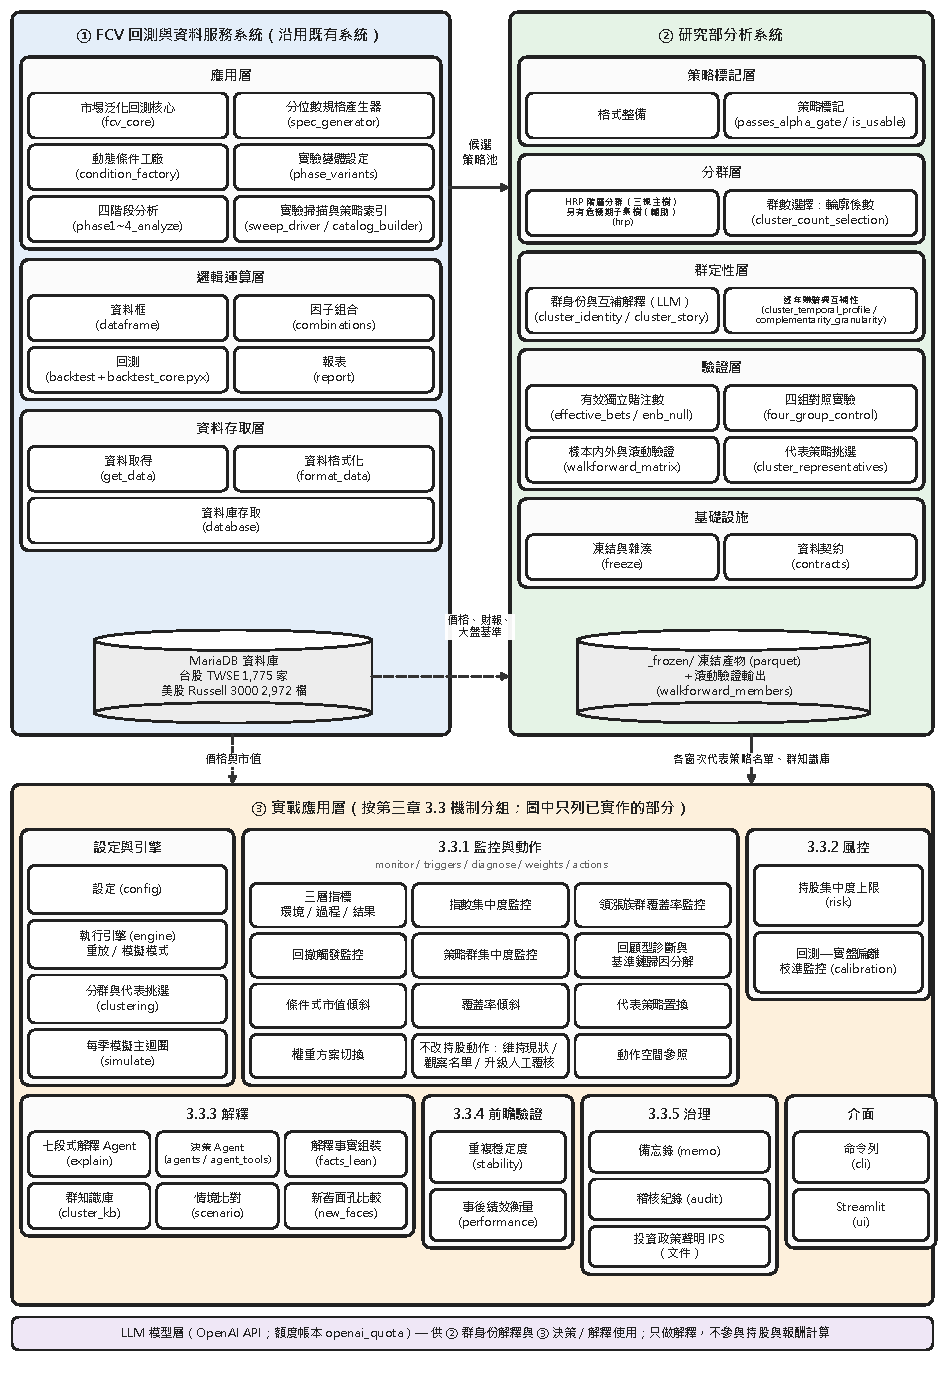
\includegraphics[width=\textwidth,height=0.88\textheight,keepaspectratio]{fig_architecture.pdf}
  \caption{系統架構圖}\label{fig:architecture}
\end{figure}

%--------------------------------------------------------------
\section{FCV 聲明式多因子回測引擎}\label{sec:fcv}
\pending{3-1：以 2-1 的因子文獻為基礎，簡短說明 FCV 引擎如何系統性產出候選策略池；篇幅精簡（這是工具，不是本章重點）。}

%--------------------------------------------------------------
\section{研究部：策略池的定性與定量分析方法論}\label{sec:research}
\pending{3-2：面對龐大的策略池，建立回答 SQ1、SQ2 所需的量化分析方法論（HRP 分群、群定性、逐年賺賠與互補性、多組對照實驗，以及從群結構決斷出最終持倉）。}

\begin{figure}[htbp]
  \centering
  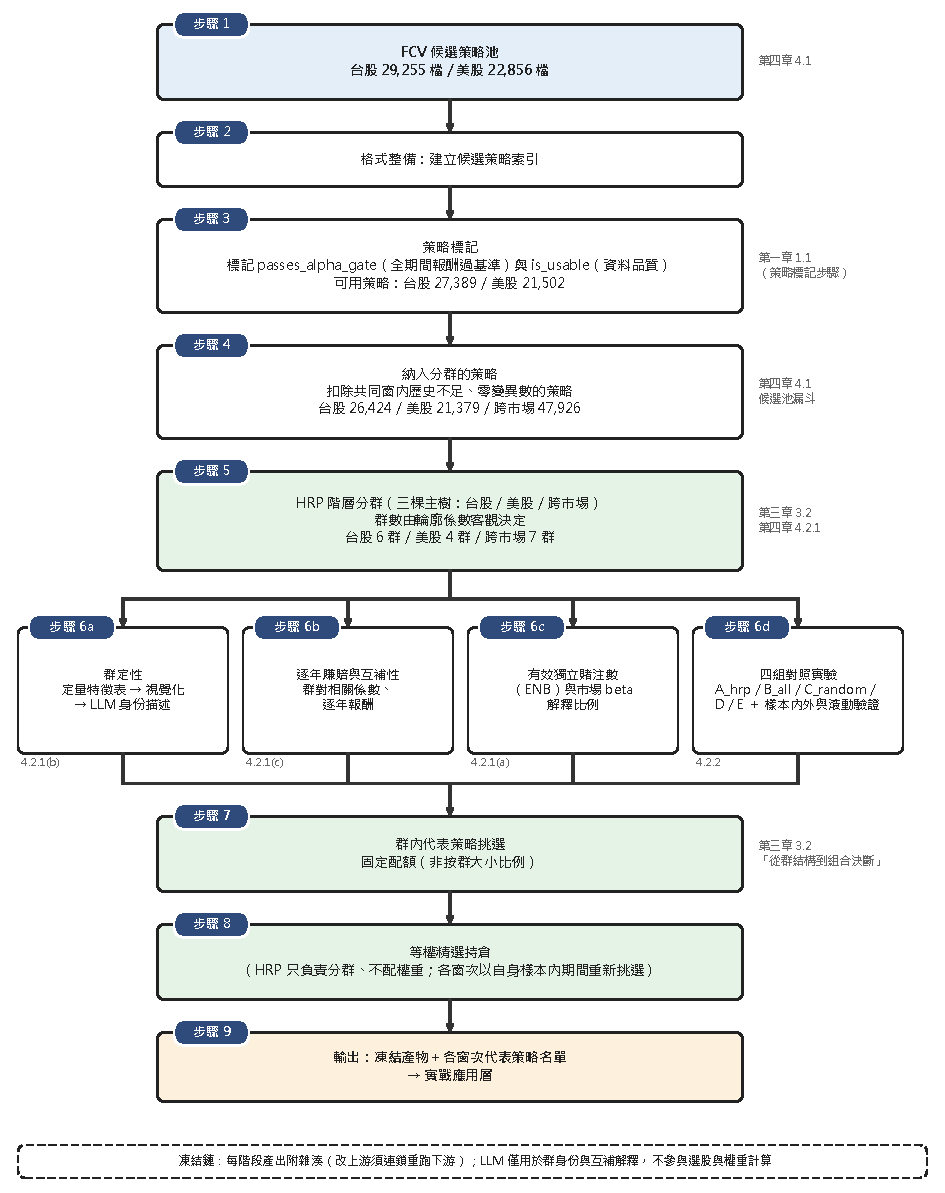
\includegraphics[width=\textwidth,height=0.88\textheight,keepaspectratio]{fig_research_flow.pdf}
  \caption{研究部建構流程}\label{fig:research-flow}
\end{figure}

%--------------------------------------------------------------
\section{監控決策系統設計}\label{sec:app}
\pending{3-3 開場：本節為本論文的核心貢獻——讓一大批機器生成的策略能被持續以樣本外監控、隔離近期偏離並執行修正。}

\subsection{核心監控與動作機制}\label{sec:monitor}
\pending{3-3-1：樣本外監控＋修正這個一般能力先講，市值集中度當具體案例後講；列出完整的監控與動作清單（見表「實戰層機制名稱對照表」）。}

\begin{figure}[htbp]
  \centering
  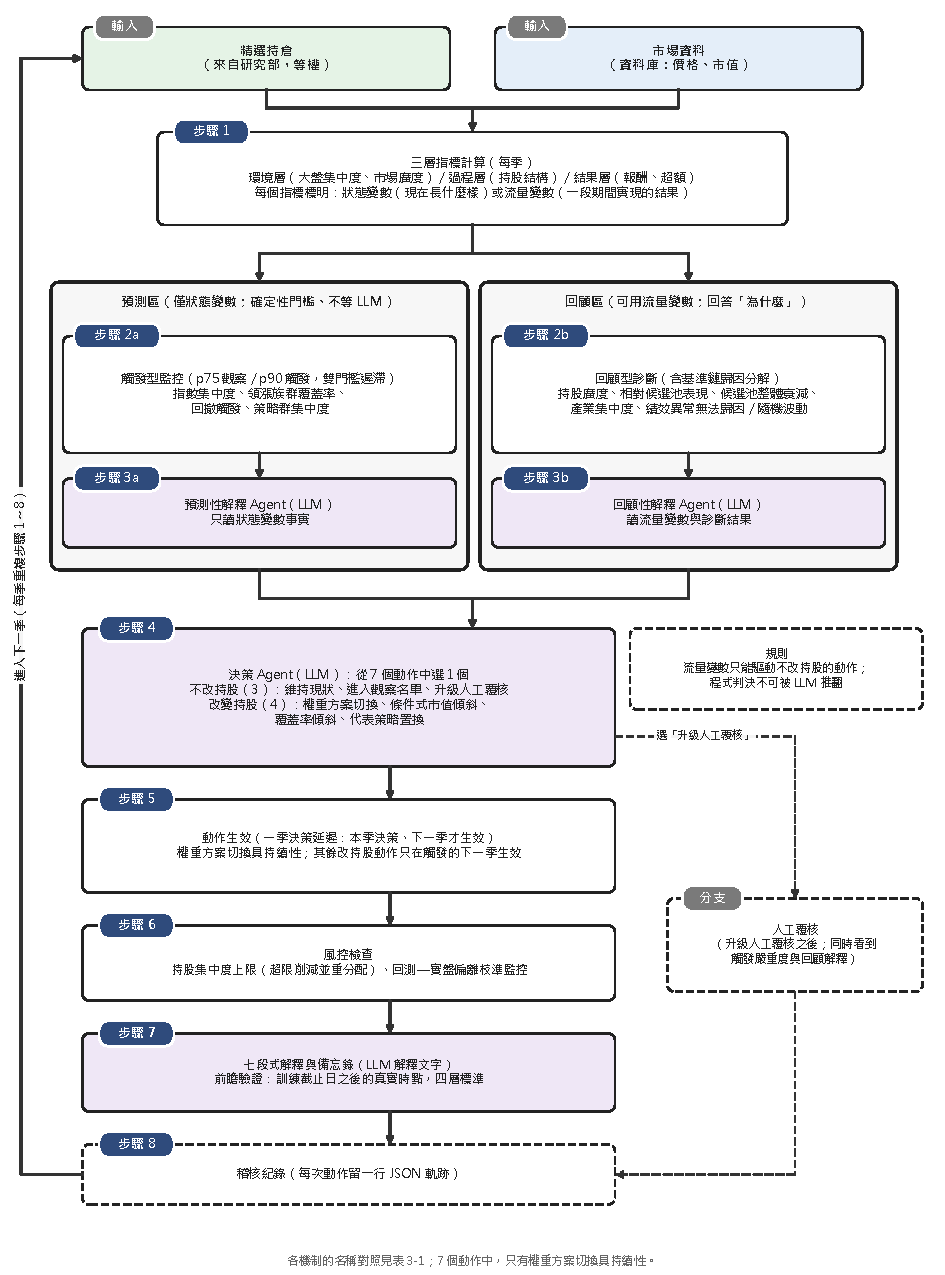
\includegraphics[width=\textwidth,height=0.88\textheight,keepaspectratio]{fig_quarterly_loop.pdf}
  \caption{每季監控決策迴圈}\label{fig:quarterly-loop}
\end{figure}

\subsection{風控層}\label{sec:risk}
\pending{3-3-2：持股集中度上限、回測—實盤偏離校準監控；須誠實交代單標的上限的調整歷程與全樣本前視偏誤。}

\subsection{解釋機制}\label{sec:explain}
\pending{3-3-3：七段式輸出結構、抗幻覺三鐵則、名詞定義（市場狀態標籤、危機期子集樹、危機期共跌）。}

\subsection{前瞻驗證}\label{sec:forward}
\pending{3-3-4：以訓練截止日之後的真實時點驗證解釋機制；四層驗證標準；LLM 影響範圍澄清。}

\subsection{法人治理設計元素}\label{sec:governance}
\pending{3-3-5：IPS、備忘錄、稽核紀錄、快慢時鐘拆分；誠實標註尚無獨立量化驗證。}

\subsection{設計項目與驗證章節對照表}\label{sec:mapping}
\pending{3-3-6：每個設計機制對應第四章哪一節、證據強度如何。}
